\apendice{Especificación de diseño}

\section{Introducción}
Los apartados que se estudiarán en esta sección son los siguientes:
\begin{itemize}
\item \textbf{Diseño de datos}
\item \textbf{Diseño procedimental}
\item \textbf{Diseño arquitectónico}
\end{itemize}
\section{Diseño de datos}
\subsection{Diseño de base de datos geo-espacial}
Como se ha comentado en puntos anteriores, se ha utilizado una base de datos geo-espacial, más específicamente \textit{OpenStreetMaps}.
Debido a que los nuevos algoritmos no solo necesitan datos referentes a los puntos y su posición, sino que requieren de las ventanas de tiempo de los establecimientos, se ha añadido una columna adicional que contenga esta información.

Respecto al resto de la estructura de la base de datos, se ha utilizado la implementada en versiones anteriores de este proyecto.

\subsubsection{Modelo de datos}
\textit{AC: Decir que se ha cambiado X para implementar las ventanas de tiempo}
\subsubsection{Tablas}
\textit{AC: Parecido a lo anterior}
\subsection{Estructura de paquetes (Servidor)}
Como en versiones anteriores del proyecto, los paquetes del servidor se encuentran divididos en dos secciones claras:
\begin{itemize}
\item Main
\item Test
\end{itemize}
Cada uno de estas secciones contienen a su vez sub-paquetes, de los que se destacarán a continuación aquellos en los que se han realizado cambios para implementar la funcionalidad correspondiente a el calculo de rutas teniendo en cuenta las ventanas de tiempo.

\subsubsection{Paquete \textit{main}}
Se trata del paquete principal de la aplicación, que a su vez contiene 7 \textbf{AC: Cambiar numero y paquetes} paquetes más.
Estos paquetes son: \textit{algorithms, crypt, database, model, performance, resource, resource.request, resource.response, router, util}

\subsubsection{Paquete algorithmsTW}

\subsubsection{Paquete modelTW}

\subsubsection{Paquete \textit{test}}
Este paquete contiene los test unitarios realizados para llevar un buen control del funcionamiento de los algoritmos.
\subsection{Diagrama de despliegue}
En este apartado se muestra el diagrama de despliegue de la aplicación.
Cabe destacar que debido a que el funcionamiento de la aplicación es el mismo que en los proyectos anteriores, también lo es el diagrama de despliegue.

Podemos dividir dicho funcionamiento en tres bloques:
\begin{itemize}
\item \textbf{Lanzamiento de petición (cliente)}: el cliente hará una petición dese la aplicación a través de una petición REST.
\item \textbf{Atención de la petición:} la petición será atendida por un \textit{servlet} ejecutándose en un contenedor de aplicaciones \textit{Glassfish}.
\item \textbf{Consulta}: Para atender la petición, el servidor realizará una consulta a una base de datos \textit{PostgreSQL}, a través de un conector \textit{JDBC}.
\end{itemize}
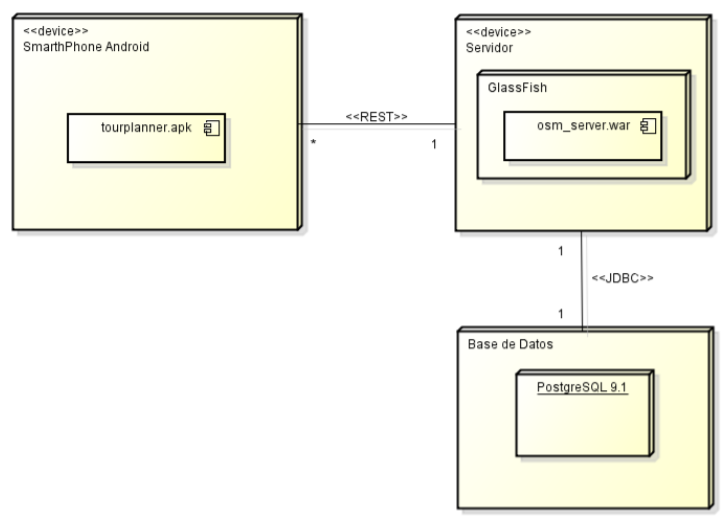
\includegraphics[width=\textwidth]{C3_DiagramaDespliegue}
\section{Diseño procedimental}
\textbf{AC: Preguntar a bruno que pongo yo aqui}
\section{Diseño arquitectónico}
\subsection{Patrón Strategy}
El patrón Strategy (Estrategia en español) es un patrón de diseño que pertenece a la categoría de \textit{behavioral patterns} (patrones de comportamiento), cuya función es identificar patrones de comunicaciones entre diferentes objetos y realizar correctamente el intercambio de mensajes entre ellos.

El patrón Strategy permite encapsular los algoritmos en clases y elegir cual queremos utilizar en tiempo de ejecución.

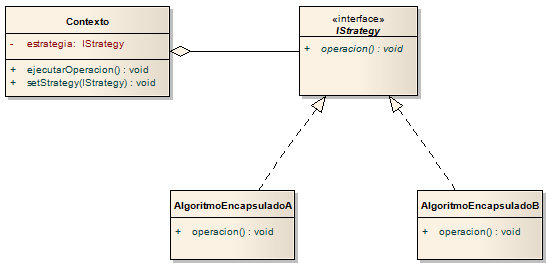
\includegraphics[width=\textwidth]{C3_PatronStrategy}

Este patrón se ha utilizado para seleccionar que algoritmo queremos que se ejecute : Chao et al, GRASP, Iterativo, Colonia de hormigas o Genético.

